\documentclass[dvipsnames,handout]{beamer} % Use handout option to remove pauses.
\usetheme{default}
\usefonttheme{structurebold}
\usefonttheme[onlymath]{serif}
\usepackage[UKenglish,cleanlook]{isodate}                                  % Set default date and date display
\usepackage[T1]{fontenc}
% Slide title background color
\definecolor{background}{HTML}{ede6d8}
% Slide title text color
\definecolor{titleText}{HTML}{B40404}
% Add slide numbers in bottom right corner
\defbeamertemplate{headline}{my header}{
    \vskip1pt
    \makebox[0pt][l]{\,\insertsection}
    \hspace*{\fill}\insertshorttitle\hspace*{\fill}
    \llap{\insertframenumber\,/\,\inserttotalframenumber\,}
}
\setbeamertemplate{headline}[my header]
% Add name at the bottom
\setbeamercolor{footlinecolor}{fg=black,bg=background}
\defbeamertemplate{footline}{my footer}{%
    \begin{beamercolorbox}[wd=\paperwidth,leftskip=0.25cm,rightskip=0.25cm]{footlinecolor}
    \hfill
    \insertshortauthor
    \end{beamercolorbox}
}
\setbeamertemplate{footline}[my footer]
\setbeamertemplate{navigation symbols}[default]
\usepackage{graphicx}
% Set font sizes for frame title and subtitle
\setbeamerfont{frametitle}{size=\fontsize{15}{16}}
\setbeamerfont{framesubtitle}{size=\small}
% Set left and right text margins
\setbeamersize{text margin left=5mm, text margin right=5mm}
\usepackage{booktabs,multirow}
\usepackage{subcaption}   % Sub figures.
\usepackage{tikz}
\usetikzlibrary{shapes,decorations,decorations.pathreplacing,arrows,calc,arrows.meta,fit,positioning}
\tikzset{
    auto,node distance =1 cm and 1 cm,semithick,
    state/.style ={ellipse, draw, minimum width = 0.7 cm},
    point/.style = {circle, draw, inner sep=0.04cm,fill,node contents={}},
    bidirected/.style={Latex-Latex,dashed},
    el/.style = {inner sep=2pt, align=left, sloped}
}
\usepackage{mathtools}                                                     % Various maths functions
\usepackage{amssymb}                                                       % Various maths functions
\usepackage{amsmath}                                                       % Various maths functions
\usepackage{dsfont}                                                        % Various maths functions
\usepackage{centernot}                                                     % center \not usage
\usepackage{siunitx} \sisetup{round-mode=places, round-precision=3}        % Formalise use of units and numbers among text
\usepackage[normalem]{ulem} % Strike-through package
\renewcommand{\vec}[1]{\boldsymbol{\mathit{#1}}}                           % vector notation shortcut
\newcommand{\mat}[1]{\boldsymbol{\mathit{#1}}}                             % matrix notation shortcut
\DeclarePairedDelimiter\abs{\lvert}{\rvert}                                % absolute value notation shortcut
\DeclarePairedDelimiter\norm{\lVert}{\rVert}                               % norm notation shortcut
\newcommand{\Prob}[1]{\Pr\left( #1 \right)}                         % SHortcut for probability notation
\newcommand{\Probgiven}[2]{\Pr\left( #1 \, \middle\vert \, #2 \right)} % SHortcut for probability notation, given
\newcommand{\E}[2][]{\mathbb{E}_{#1} \left[ #2 \right]}                    % Expectation (with optional subscript) shortcut
\newcommand{\Egiven}[3][]{\mathbb{E}_{#1} \left[ #2 \, \middle\vert \, #3 \right]} % Expectation given (with optional subscript) shortcut
\newcommand{\Var}[2][]{\text{Var}_{#1} \left( #2 \right)}                  % Variation (with optional subscript) shortcut
\newcommand{\Cov}[1]{\text{Cov} \left( #1 \right)}                         % Covariance (with optional subscript) shortcut
\newcommand{\indicator}[1]{\mathds{1}\left\{ #1 \right\}}                  % SHortcut for indicator function
\newcommand{\indep}{\, \raisebox{0.05em}{\rotatebox[origin=c]{90}{$\models$}} \,}% Statistical independence symbol.
\newcommand{\diff}[2][]{\frac{d#1}{d#2}}                                   % SHortcut for differential fraction as a function
\newcommand{\partialdiff}[2][]{\frac{\partial#1}{\partial#2}}              % SHortcut for partial differential fraction as a function
\renewcommand{\hat}[1]{\widehat{#1}}                                       % Default estimator notation is widehat
\renewcommand{\bar}[1]{\overline{#1}}                                      % Make over bar look nicer
\renewcommand{\tilde}[1]{\widetilde{#1}}                                   % Make over tilde look better
% Citations
\usepackage{natbib}                                        % Citation package, see https://en.wikibooks.org/wiki/LaTeX/Bibliography_Management#Natbib
\usepackage{hyperref}                                        % Allow for links across the text, with colour options
\usepackage{setspace}    
\usepackage{soul,color,xcolor} % Text highlighting
\makeatletter
\let\HL\hl
\renewcommand\hl{%
    \let\set@color\beamerorig@set@color
    \let\reset@color\beamerorig@reset@color
    \HL}
\makeatother
\newcommand{\mathcolorbox}[2]{\colorbox{#1}{$\displaystyle #2$}}
% Set colors
\setbeamercolor{block title}{use=structure,fg=white,bg=structure.fg!75!black}
\setbeamercolor{block body}{parent=normal text,use=block title,bg=block title.bg!10!bg}
\setbeamercovered{transparent}
\setbeamercolor{postit}{fg=black, bg=yellow}
\setbeamercolor{frametitle}{bg=background, fg=titleText}
\setbeamercolor{subtitle}{fg=titleText}
% Command to align text
\renewcommand{\raggedright}{\leftskip=0pt \rightskip=0pt plus 0cm}

%-------------------------------------------------------------------------------
% Title Page
%-------------------------------------------------------------------------------
\title{\color{titleText}
    Causal Mediation in Natural Experiments
}
\author[Senan Hogan-Hennessy, Cornell University]{
    Senan Hogan-Hennessy \\
    Economics Department, Cornell University \\ %\vspace{0.5cm}
    \href{mailto:seh325@cornell.edu}{\textcolor{blue}{seh325@cornell.edu}}
}
\date{} % Date, can be changed to a custom date

%-------------------------------------------------------------------------------
% Opening Slides
\begin{document}
% Justify text through-out.
\raggedright
%-------------------------------------------------------------------------------
%% Title page
\begin{frame}[noframenumbering, plain]
    % Print the title page as the first slide
    \titlepage
    \vspace{-1.5cm}
    \begin{center}
        
\includegraphics[width=2cm]{presentation-files/cornell}

        \vspace{0.5cm}
        Labour Work in Progress Seminar \\
        6 March 2025
    \end{center}
\end{frame}

%-------------------------------------------------------------------------------
% Plan
\begin{frame}[noframenumbering, plain]
    \frametitle{Plan}
    \begin{enumerate}
        \item Start with explaining natural experiment, good for ATE $Z \to Y$.
        COnsider the Oregon health insurance experiment, or Vietnam draft instrument.
        \item Does not illuminate how these causal effects came about.
        \item You may have read epidemiology, medicine, or psychology and wondered what these claims are ``mediated through.''
        \item These are mediation effect estimates, and they estimate ``how much of the ATE goes through this channel?  How much is left-over?''
        \item Leads to my introduction page. 
    \end{enumerate}
\end{frame}

%-------------------------------------------------------------------------------
% Introduction.
\section{Introduction}
%-------------------------------------------------------------------------------
\begin{frame}
    \frametitle{Introduction}
    \begin{figure}[h!]
        \centering
        \singlespacing
        \begin{subfigure}[c]{\textwidth}
            Have you ever read an epidemiology/psychology/medicine paper's abstract, and seen claims of mediator effects \textbf{mediated} through some mechanism?
        \end{subfigure}
        \begin{subfigure}[c]{0.75\textwidth}
            \centering
            \singlespacing
            \begin{subfigure}[c]{\textwidth}
                \centering
                
\includegraphics[width=\textwidth]{presentation-files/headlines/rangarajan-2006.png}
            \end{subfigure}
        \end{subfigure}
    \end{figure}
\end{frame}
%-------------------------------------------------------------------------------
\begin{frame}[noframenumbering]
    \frametitle{Introduction}
    \begin{figure}[h!]
        \centering
        \singlespacing
        \begin{subfigure}[c]{\textwidth}
            Have you ever read an epidemiology/psychology/medicine paper's abstract, and seen claims of mediator effects \textbf{mediated} through some mechanism?
        \end{subfigure}
        \begin{subfigure}[c]{0.75\textwidth}
            \centering
            \singlespacing
            \begin{subfigure}[c]{\textwidth}
                \centering
                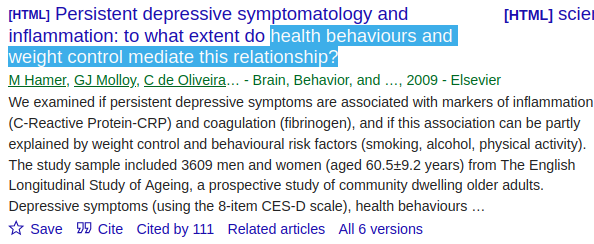
\includegraphics[width=\textwidth]{presentation-files/headlines/hamer-2009.png}
            \end{subfigure}
        \end{subfigure}
    \end{figure}
\end{frame}
%-------------------------------------------------------------------------------
\begin{frame}[noframenumbering]
    \frametitle{Introduction}
    \begin{tabular}{l l}
        \textbf{1980s:}
        & Psychometrics defined mediation (distinct from moderation). \\
        \textbf{1920s:} 
        & Application of early econometric path analysis (Wright 1928). \\
        \textbf{2020s:}
        & Popular in epidemiology, medicine, psychology.
    \end{tabular}
    \vskip-0.5cm
    \begin{figure}
        \centering
        \singlespacing
        \caption{Baron Kelly (1986), p. 1176.}
        \vskip-0.25cm
        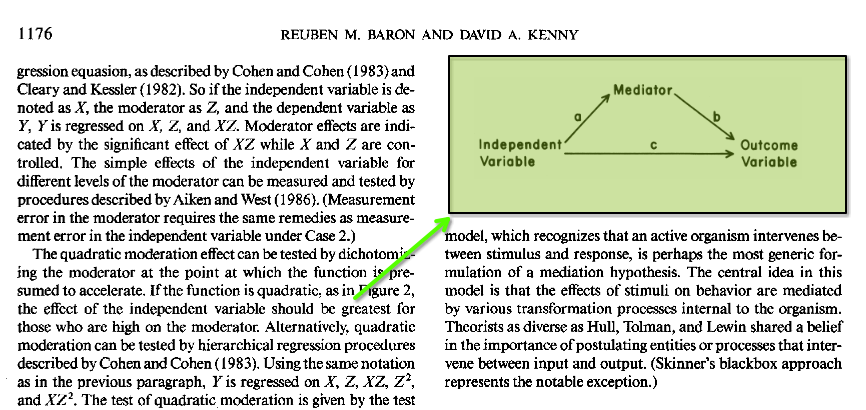
\includegraphics[width=0.9\textwidth]{presentation-files/headlines/baronkelly-1986.png}
    \end{figure}
\end{frame}%-------------------------------------------------------------------------------
\begin{frame}[noframenumbering]
    \frametitle{Introduction:}
    \begin{enumerate}
        \item \textbf{[familiar]} Causal design to estimate a treatment effect.
        \begin{figure}
            \centering
            \singlespacing
            \vspace{-0.5cm}
            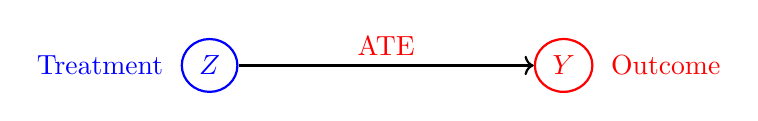
\begin{tikzpicture}
                \node[state, thick,blue] (treatment) at (0,0) {$Z$};
                \node[state, thick,red] (outcome) [right=3.75cm of treatment] {$Y$};
                \path[->, thick] (treatment) edge (outcome);
                % Label the nodes with econ examples
                \node[color=blue, left=0.1cm of treatment] {Treatment};
                \node[color=red, right=0.1cm of outcome] {Outcome};
                % Label the effect in the middle
                \path (treatment) -- (outcome) node[midway] (label) {};
                \node[color=red, above=-0.25cm of label] {ATE};
            \end{tikzpicture}
        \end{figure}
        \item \textbf{[unfamiliar]} CM decomposes ATE along a mechanism pathway.
        \begin{figure}
            \centering
            \singlespacing
            \vspace{-0.5cm}
            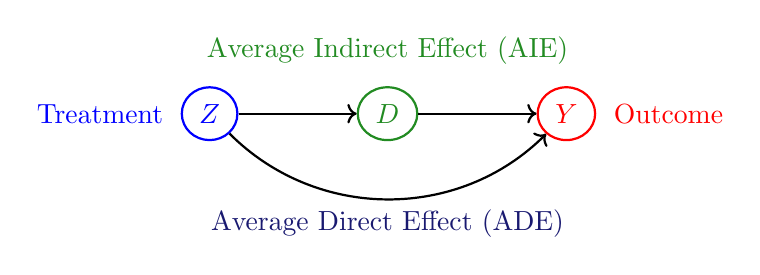
\begin{tikzpicture}
                \node[state, thick,ForestGreen] (mediator) at (0,0) {$D$};
                \node[state, thick,blue] (treatment) [left=1.5cm of mediator] {$Z$};
                \node[state, thick,red] (outcome) [right=1.5cm of mediator] {$Y$};
                %\path[->,thick] (treatment) edge (mediator);
                %\path[->,thick] (mediator) edge (outcome);
                % Label the nodes with econ examples
                \node[color=blue, left=0.1cm of treatment] {Treatment};
                \node[color=red, right=0.1cm of outcome] {Outcome};
                \node[color=ForestGreen, above=0.15cm of mediator] {Average Indirect Effect (AIE)};
                % Add in direct + indirect effects.
                %\path[->,thick] (treatment) edge[bend right=45] (outcome);
                % Label the pathways with the colours
                \path[->, thick] (treatment) edge (mediator);
                \path[->, thick] (mediator) edge (outcome);
                \path[->, thick] (treatment) edge[bend right=45] (outcome);
                \node[color=MidnightBlue, below=0.75cm of mediator] {Average Direct Effect (ADE)};
            \end{tikzpicture}
        \end{figure}
        \item
        \begin{tabular}{ll}
            \textbf{ATE} & $\implies$ Average causal effect $Z \to Y$ \\
            \textbf{AIE} & $\implies$ How much $Z \to Y$ effect through mediator $D$? \\
            \textbf{ADE} & $\implies$ How much $Z \to Y$ effect is left over?
        \end{tabular}
    \end{enumerate}
\end{frame}%-------------------------------------------------------------------------------
\begin{frame}[noframenumbering]
    \frametitle{Introduction---  CM Examples:}
    \begin{enumerate}
        \item Lottery military draft 1969 (Angrist 1990).
        \begin{figure}[h!]
            \centering
            \singlespacing
            \begin{subfigure}[c]{0.3\textwidth}
                \centering
                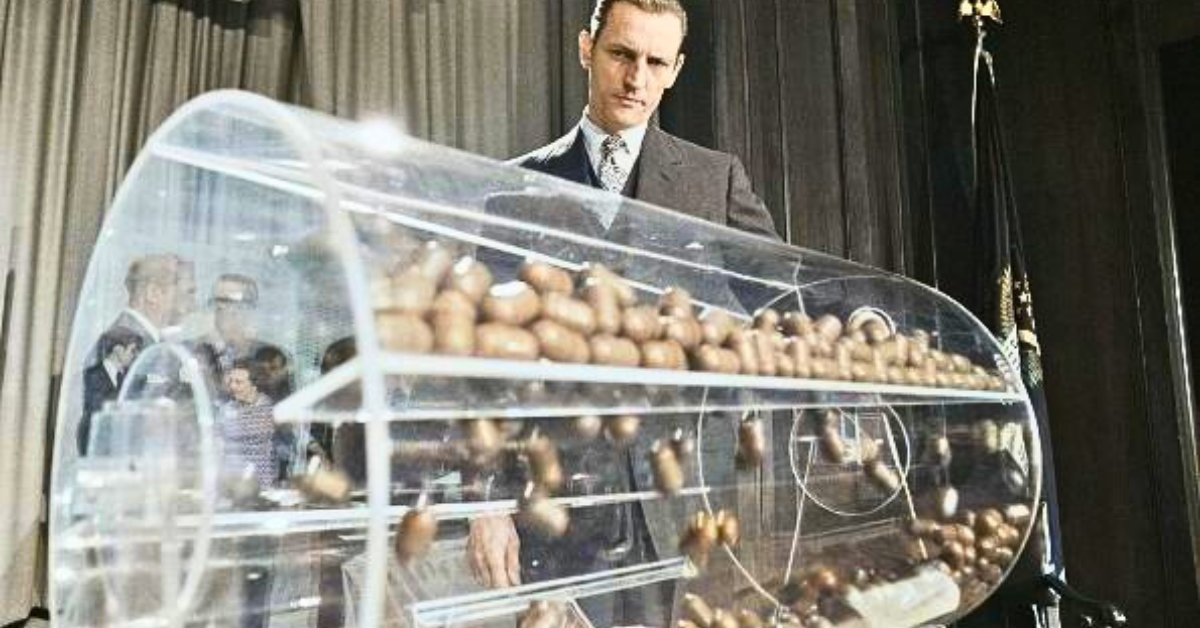
\includegraphics[width=\textwidth]{presentation-files/headlines/1969-draft-lottery.jpeg}
            \end{subfigure}
            \hspace{0.25cm}
            \begin{subfigure}[c]{0.55\textwidth}
                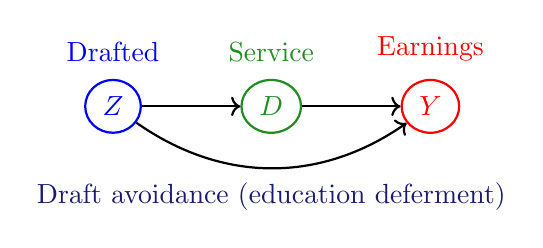
\begin{tikzpicture}
                    \node[state, thick,ForestGreen] (mediator) at (0,0) {$D$};
                    \node[state, thick,blue] (treatment) [left=1.25cm of mediator] {$Z$};
                    \node[state, thick,red] (outcome) [right=1.25cm of mediator] {$Y$};
                    %\path[->,thick] (treatment) edge (mediator);
                    %\path[->,thick] (mediator) edge (outcome);
                    % Label the nodes with econ examples
                    \node[color=blue, above=0.1cm of treatment] {Drafted};
                    \node[color=red, above=0.1cm of outcome] {Earnings};
                    \node[color=ForestGreen, above=0.1cm of mediator] {Service};
                    % Add in direct + indirect effects.
                    %\path[->,thick] (treatment) edge[bend right=45] (outcome);
                    % Label the pathways with the colours
                    \path[->, thick] (treatment) edge (mediator);
                    \path[->, thick] (mediator) edge (outcome);
                    \path[->, thick] (treatment) edge[bend right=35] (outcome);
                    \node[color=MidnightBlue, below=0.5cm of mediator] {Draft avoidance (education deferment)};
                \end{tikzpicture}
            \end{subfigure}
        \end{figure}
        \textbf{Note:} instrumental variables assumes direct $=0$ (exclusion restriction).
        \vspace{0.125cm}
        \item Oregon health insurance experiment (Finkelstein$+$ 2009).
        \vspace{-0.4cm}

        \begin{figure}[h!]
            \centering
            \singlespacing
            \begin{subfigure}[c]{0.3\textwidth}
                \centering
                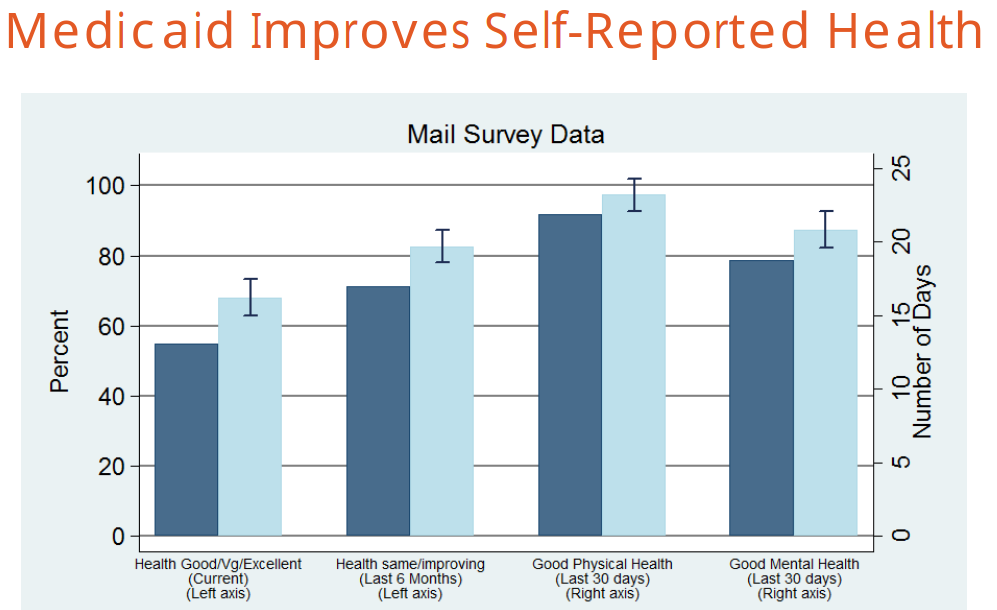
\includegraphics[width=\textwidth]{presentation-files/headlines/finkelstein-2019.png}
            \end{subfigure}
            \begin{subfigure}[c]{0.55\textwidth}
                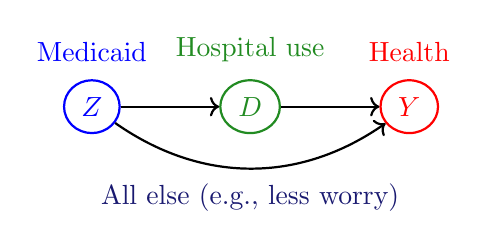
\begin{tikzpicture}
                    \node[state, thick,ForestGreen] (mediator) at (0,0) {$D$};
                    \node[state, thick,blue] (treatment) [left=1.25cm of mediator] {$Z$};
                    \node[state, thick,red] (outcome) [right=1.25cm of mediator] {$Y$};
                    % Label the nodes with econ examples
                    \node[color=blue, above=0.1cm of treatment] {Medicaid};
                    \node[color=red, above=0.1cm of outcome] {Health};
                    \node[color=ForestGreen, above=0.1cm of mediator] {Hospital use};
                    % Add in direct + indirect effects.
                    %\path[->,thick] (treatment) edge[bend right=45] (outcome);
                    % Label the pathways with the colours
                    \path[->, thick] (treatment) edge (mediator);
                    \path[->, thick] (mediator) edge (outcome);
                    \path[->, thick] (treatment) edge[bend right=35] (outcome);
                    \node[color=MidnightBlue, below=0.5cm of mediator] {All else (e.g., less worry)};
                \end{tikzpicture}
            \end{subfigure}
        \end{figure}
    \end{enumerate}
\end{frame}
%-------------------------------------------------------------------------------
\begin{frame}[noframenumbering]
    \frametitle{Introduction}
    This project examines CM methods from an economic perspective:
    \begin{enumerate}
        \item Problems with conventional, selection-on-observables, approach to CM in social science settings --- including natural experiments.
        \\ \textbf{[Negative result]}
        \item Recovering valid CM effects under selection-into-mediator, using a selection model.
        \\ \textbf{[Positive result]}
    \end{enumerate}
    \vspace{0.25cm}
    Brings together ideas from two different literatures:
    \begin{itemize}
        \item \textbf{Causal mediation.}
        \\ Baron Kelly (1986), Imai Keele Yamamoto (2010), Flores Flores-Lagunes (2009), Fr\"olich Huber (2017), Huber (2020), Kwon Roth (2024).
        \item \textbf{Selection-into-treatment, selection models/MTEs.}
        \\ Roy (1951), Heckman (1979), Heckman Honore (1990), Florens Heckman Meghir Vytlacil (2008).
    \end{itemize}
\end{frame}%-------------------------------------------------------------------------------
\section{1. Direct \& Indirect Effects}
%-------------------------------------------------------------------------------
\begin{frame}
    \frametitle{Direct \& Indirect Effects --- Model}
    Consider binary treatment $Z_i = 0, 1$,
    binary mediator $D_i = 0, 1$,
    and continuous outcome $Y_i$.
    \begin{figure}
        \centering
        \singlespacing
        \vspace{-1cm}
        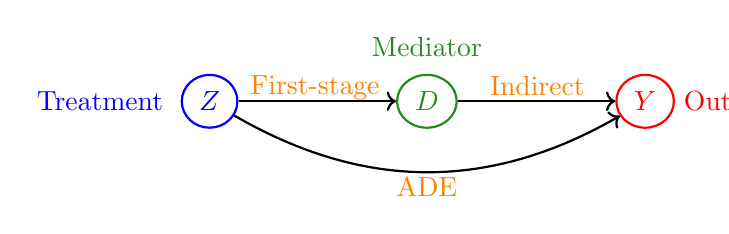
\begin{tikzpicture}
            \node[state, thick,ForestGreen] (mediator) at (0,0) {$D$};
            \node[state, thick,blue] (treatment) [left=2cm of mediator] {$Z$};
            \node[state, thick,red] (outcome) [right=2cm of mediator] {$Y$};
            % Label Z, D, Y
            \node[color=ForestGreen] [above=0.1cm of mediator] {Mediator};
            \node[color=blue] [left=0.1cm of treatment] {Treatment};
            \node[text width=0.1cm, color=red] [right=-0.01cm of outcome] {Outcome};
            % Draw the causal arrows
            \path[->, thick] (treatment) edge (mediator);
            \path[->, thick] (mediator) edge (outcome);
            \path[->, thick] (treatment) edge[bend right=30] (outcome);
            % Label direct and indirect effect
            \node[color=orange] [above left=-0.35cm and 0.2cm of mediator] {First-stage};
            \node[color=orange] [above right=-0.3cm and 0.4cm of mediator] {Indirect};
            \node[color=orange] [below=0.5cm of mediator] {ADE};
            % Add in the confounders
            %\node[state, thick,RoyalPurple] (confounderX) [above=1.5cm of mediator] {$\vec{X}$};
            %\path[->,RoyalPurple] (confounderX) edge (mediator);
            %\node[color=RoyalPurple] [left=0.1cm of confounderX] {Observed controls};
            %\node[state, thick,dashed,RoyalBlue] (confounderU) [above=0.75cm of outcome] {$\vec U$};
            %\path[->,dashed,color=RoyalBlue] (confounderU) edge (mediator);
            %\path[->,dashed,color=RoyalBlue] (confounderU) edge (outcome);
            %\node[color=RoyalBlue] [right=0.1cm of confounderU] {Unobserved confounder};
        \end{tikzpicture}
    \end{figure}
    \vspace{-0.5cm}
    \begin{align*}
        D_i& \text{ is a function of } Z_i: &
            Y_i& \text{ is a function of both } Z_i,D_i: \\
        D_i& = Z_i D_i(1) + (1 - Z_i) D_i(0). &
            Y_i& = Z_i Y_i(1, D_i(1)) + (1 - Z_i) Y_i(0, D_i(0)).
    \end{align*}
    \par\noindent\rule{\textwidth}{0.4pt}
    \pause
    Assume $Z_i$ is ignorable, conditional on $\vec X_i$.
    \[ Z_i \indep  D_i(z), Y_i(z', d) \; \; | \;\; \vec X_i \text{ for } z, z', d = 0, 1. \]
    \pause
    Only two causal effects are identified so far.
    \begin{align*}
    \text{ATE:} \;\; \E{Y_i(1, D_i(1)) - Y_i(0, D_i(0))}
        &= \Egiven{Y_i}{Z_i = 1} - \Egiven{Y_i}{Z_i = 0} \\
    \text{Average first-stage:} \;\; \E{D_i(1) - D_i(0)}
        &=\Egiven{D_i}{Z_i = 1} - \Egiven{D_i}{Z_i = 0}
    \end{align*}
\end{frame}
%-------------------------------------------------------------------------------
\begin{frame}
    \frametitle{Direct \& Indirect Effects --- Definitions}
    \vskip-1.0cm
    \begin{figure}
        \centering
        \singlespacing
        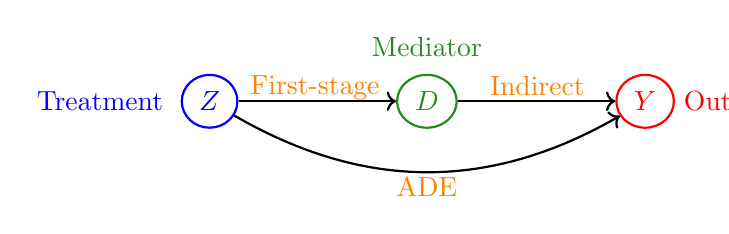
\begin{tikzpicture}
            \node[state, thick,ForestGreen] (mediator) at (0,0) {$D$};
            \node[state, thick,blue] (treatment) [left=2cm of mediator] {$Z$};
            \node[state, thick,red] (outcome) [right=2cm of mediator] {$Y$};
            % Label Z, D, Y
            \node[color=ForestGreen] [above=0.1cm of mediator] {Mediator};
            \node[color=blue] [left=0.1cm of treatment] {Treatment};
            \node[text width=0.1cm, color=red] [right=-0.01cm of outcome] {Outcome};
            % Draw the causal arrows
            \path[->, thick] (treatment) edge (mediator);
            \path[->, thick] (mediator) edge (outcome);
            \path[->, thick] (treatment) edge[bend right=30] (outcome);
            % Label direct and indirect effect
            \node[color=orange] [above left=-0.35cm and 0.2cm of mediator] {First-stage};
            \node[color=orange] [above right=-0.3cm and 0.4cm of mediator] {Indirect};
            \node[color=orange] [below=0.5cm of mediator] {ADE};
            % Add in the confounders
            %\node[state, thick,RoyalPurple] (confounderX) [above=1.5cm of mediator] {$\vec{X}$};
            %\path[->,RoyalPurple] (confounderX) edge (mediator);
            %\node[color=RoyalPurple] [left=0.1cm of confounderX] {Observed controls};
            %\node[state, thick,dashed,RoyalBlue] (confounderU) [above=0.75cm of outcome] {$\vec U$};
            %\path[->,dashed,color=RoyalBlue] (confounderU) edge (mediator);
            %\path[->,dashed,color=RoyalBlue] (confounderU) edge (outcome);
            %\node[color=RoyalBlue] [right=0.1cm of confounderU] {Unobserved confounder};
        \end{tikzpicture}
    \end{figure}
    \vspace{-0.75cm}
    
    \textbf{Definitions:}
    \begin{align*}
        \text{Average Direct Effect (ADE)}: \;\;\;&
            \E{Y_i(1, D_i(Z_i)) - Y_i(0, D_i(Z_i))}, \\
        \text{Average Indirect Effect (AIE):} \;\;\;&
                \E{Y_i(Z_i, D_i(1)) - Y_i(Z_i, D_i(0))}.
    \end{align*}
    \vfill
    \begin{itemize}
        \item ADE is average effect $Z\to Y$, blocking the $D$ path.
        \item AIE is causal effect of $D \to Y$, times number of $D(Z)$ compliers.\footnote[frame]{
            Assume mediator monotonicity to simplify notation.}
    \end{itemize}
    \[ \text{AIE } =
    \E{D_i(1) -D_i(0)} \Egiven{Y_i(Z_i, 1) - Y_i(Z_i, 0)}{D_i(1) =1, D_i(0) = 0}. \]
\end{frame}
%-------------------------------------------------------------------------------
\begin{frame}
    \frametitle{Direct \& Indirect Effects --- Identification} 
    \textbf{Sequential ignorability} (\textbf{SI}, Imai Keele Yamamoto 2010):
    \vskip0.125cm
    Assume mediator $D_i$ is \textit{also} ignorable, conditional on $\vec X_i$ and $Z_i$ realisation
    \[ D_i \indep Y_i(z', d) \;\; | \;\; \vec X_i, Z_i = z',
    \text{ for } z', d = 0, 1. \]
    \par\noindent\rule{\textwidth}{0.4pt}
    \pause
    If \textbf{SI} holds then ADE and AIE are identified by two-stage regression:
    \begin{align*}
        \text{ADE} &= \E{
            \underbrace{\Egiven{Y_i}{Z_i = 1, D_i = d', \vec X_i} - \Egiven{Y_i}{Z_i = 0, D_i = d', \vec X_i}}_{\text{Second-stage regression, $Y_i$ on $Z_i$ holding $D_i, \vec X_i$ constant}}} \\
        \text{AIE} &= \E{
            \begin{aligned}
                & \underbrace{\Big(\Egiven{D_i}{Z_i = 1, \vec X_i} - \Egiven{D_i}{Z_i = 0, \vec X_i} \Big)}_{\text{First-stage regression, $D_i$ on $Z_i$}} \\
                & \times \underbrace{\Big(
                    \Egiven{Y_i}{Z_i = z', D_i = 1, \vec X_i} - \Egiven{Y_i}{Z_i = z', D_i = 0, \vec X_i} \Big)}_{\text{Second-stage regression, $Y_i$ on $D_i$ holding $Z_i, \vec X_i$ constant}}
            \end{aligned}}
    \end{align*}
\end{frame}
%-------------------------------------------------------------------------------
\begin{frame}[noframenumbering]
    \frametitle{Direct \& Indirect Effects --- Identification} 
    \textbf{Sequential ignorability} (\textbf{SI}, Imai Keele Yamamoto 2010):
    \vskip0.125cm
    Assume mediator $D_i$ is \textit{also} ignorable, conditional on $\vec X_i$ and $Z_i$ realisation
    \[ D_i \indep Y_i(z', d) \;\; | \;\; \vec X_i, Z_i = z',
    \text{ for } z', d = 0, 1. \]
    \par\noindent\rule{\textwidth}{0.4pt}
    E.g., OLS simultaneous regression (Imai Keele Yamamoto, 2010):
    \begin{align*}
        &\textcolor{blue}{Z_i \leftarrow \text{ Treatment}} &
        \text{First-stage: }
            \textcolor{ForestGreen}{D_i}
                &= \phi + \pi \textcolor{blue}{Z_i} + \vec \psi_1' \vec X_i + \eta_i \\
        &\textcolor{ForestGreen}{D_i \leftarrow \text{ Mediator}} &
        \text{Second-stage: }
            \textcolor{red}{Y_i}
                &= \alpha
                    + \beta \textcolor{ForestGreen}{D_i}
                    + \gamma \textcolor{blue}{Z_i}
                    + \delta \textcolor{blue}{Z_i} \textcolor{ForestGreen}{D_i}
                    + \vec \psi_2' \vec X_i
                    + \varepsilon_i \\
        &\textcolor{red}{Y_i \leftarrow \text{ Outcome}} &
            \implies \textcolor{Orange}{\text{ADE }}
            &= \gamma + \delta \E{\textcolor{ForestGreen}{D_i}} \\
        &   &\textcolor{Orange}{\text{AIE }}
            &= \pi \left( \beta + \delta \E{\textcolor{blue}{Z_i}} \right)
    \end{align*}
    i.e., a regression decomposition.

    \vfill
    Other estimation methods do the same decomposition, avoiding linearity assumptions (see Huber 2020 for an overview).
\end{frame}
%-------------------------------------------------------------------------------
\begin{frame}
    \frametitle{Direct \& Indirect Effects --- Selection} 
    $\implies$ Great, we can use the Imai Keele Yamamoto (2010) approach to CM all our respective applied projects.

    $\implies$ Learn the mechanism pathways in causal research
    $\to$ big gain!
    \par\noindent\rule{\textwidth}{0.4pt}

    Before we join epidemiologists/psychologists/medical researchers in this conclusion, let us interrogate the \textbf{SI} assumption.
    \[ D_i \indep Y_i(z', d) \;\; | \;\; \vec X_i, Z_i = z',
    \text{ for } z', d = 0, 1. \]
    \colorbox{yellow}{Would this assumption hold true in settings that social scientists consider?}
    \par\noindent\rule{\textwidth}{0.4pt}
    \pause  
    Return to the Oregon health insurance experiment (Finkelstein$+$ 2009).
    \vspace{-0.4cm}

    \begin{figure}[h!]
        \centering
        \singlespacing
        \begin{subfigure}[c]{0.3\textwidth}
            \centering
            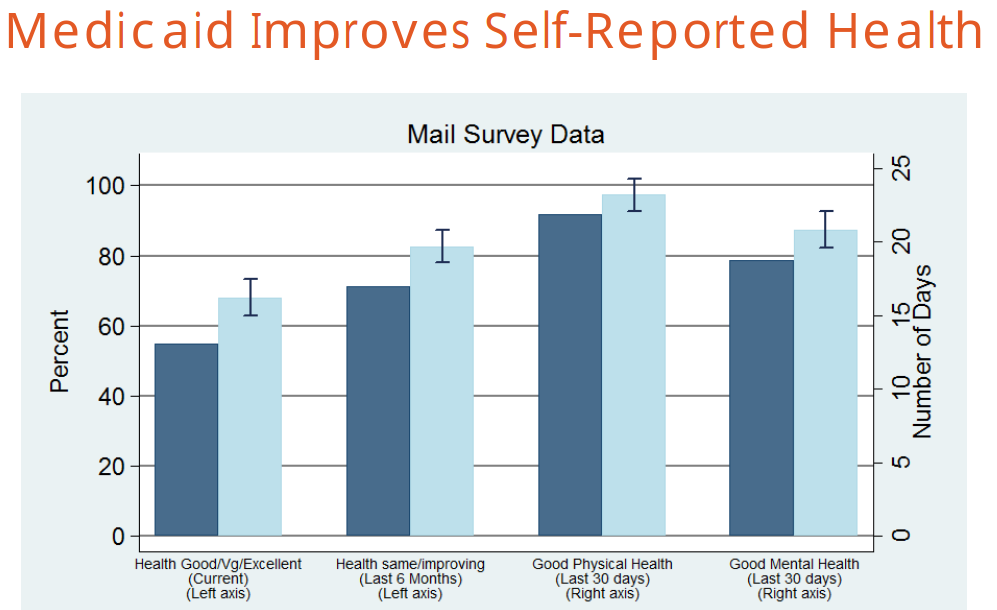
\includegraphics[width=\textwidth]{presentation-files/headlines/finkelstein-2019.png}
        \end{subfigure}
        \begin{subfigure}[c]{0.55\textwidth}
            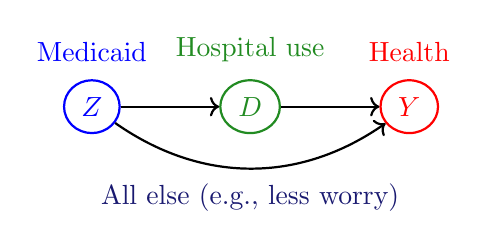
\begin{tikzpicture}
                \node[state, thick,ForestGreen] (mediator) at (0,0) {$D$};
                \node[state, thick,blue] (treatment) [left=1.25cm of mediator] {$Z$};
                \node[state, thick,red] (outcome) [right=1.25cm of mediator] {$Y$};
                % Label the nodes with econ examples
                \node[color=blue, above=0.1cm of treatment] {Medicaid};
                \node[color=red, above=0.1cm of outcome] {Health};
                \node[color=ForestGreen, above=0.1cm of mediator] {Hospital use};
                % Add in direct + indirect effects.
                %\path[->,thick] (treatment) edge[bend right=45] (outcome);
                % Label the pathways with the colours
                \path[->, thick] (treatment) edge (mediator);
                \path[->, thick] (mediator) edge (outcome);
                \path[->, thick] (treatment) edge[bend right=35] (outcome);
                \node[color=MidnightBlue, below=0.5cm of mediator] {All else (e.g., less worry)};
            \end{tikzpicture}
        \end{subfigure}
    \end{figure}
\end{frame}
%-------------------------------------------------------------------------------
\begin{frame}[noframenumbering]
    \frametitle{Direct \& Indirect Effects --- Selection} 
    \[ \text{\textbf{SI}:} \;\;\;\;\;\;\;\;\;
    D_i \indep Y_i(z', d) \;\; | \;\; \vec X_i, Z_i = z',
    \text{ for } z', d = 0, 1. \]
    Oregon health insurance experiment (Finkelstein$+$ 2009).
    \vspace{-0.4cm}

    \begin{figure}[h!]
        \centering
        \singlespacing
        \begin{subfigure}[c]{0.3\textwidth}
            \centering
            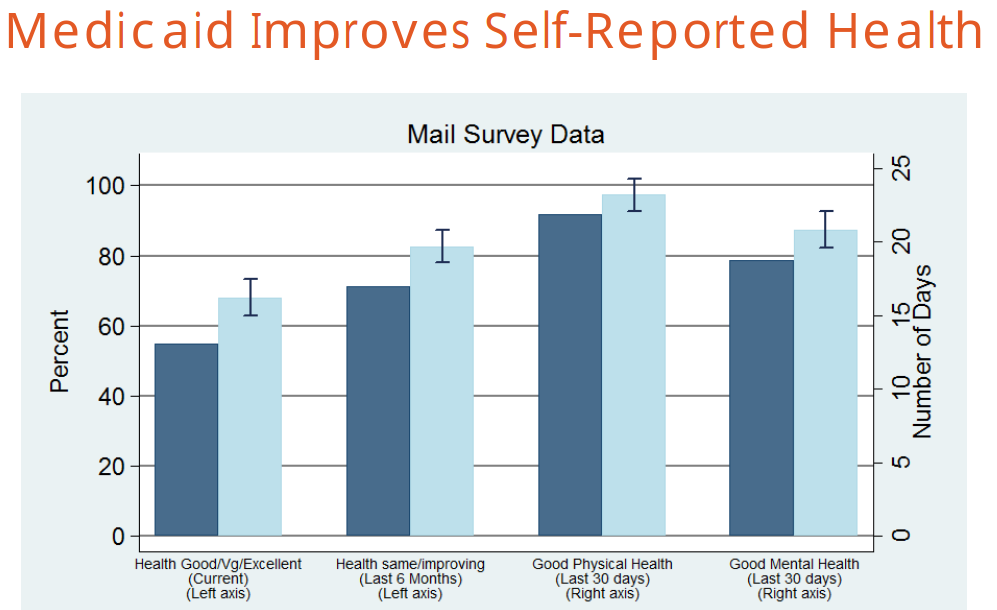
\includegraphics[width=\textwidth]{presentation-files/headlines/finkelstein-2019.png}
        \end{subfigure}
        \begin{subfigure}[c]{0.55\textwidth}
            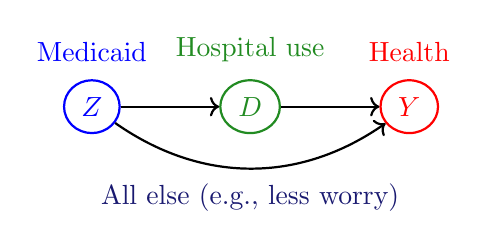
\begin{tikzpicture}
                \node[state, thick,ForestGreen] (mediator) at (0,0) {$D$};
                \node[state, thick,blue] (treatment) [left=1.25cm of mediator] {$Z$};
                \node[state, thick,red] (outcome) [right=1.25cm of mediator] {$Y$};
                % Label the nodes with econ examples
                \node[color=blue, above=0.1cm of treatment] {Medicaid};
                \node[color=red, above=0.1cm of outcome] {Health};
                \node[color=ForestGreen, above=0.1cm of mediator] {Hospital use};
                % Add in direct + indirect effects.
                %\path[->,thick] (treatment) edge[bend right=45] (outcome);
                % Label the pathways with the colours
                \path[->, thick] (treatment) edge (mediator);
                \path[->, thick] (mediator) edge (outcome);
                \path[->, thick] (treatment) edge[bend right=35] (outcome);
                \node[color=MidnightBlue, below=0.5cm of mediator] {All else (e.g., less worry)};
            \end{tikzpicture}
        \end{subfigure}
    \end{figure}
    \textbf{SI} in this setting:
    \begin{enumerate}
        \item Health insurance assigned randomly (ensured by studying the 2008 Oregon waitlist lottery).
        \item \colorbox{yellow}{Hospital usage is quasi-random, conditional on Medicaid assignment $Z_i$} \\
        \colorbox{yellow}{and demographics $\vec X_i$.}

    \end{enumerate}
\end{frame}
%-------------------------------------------------------------------------------
\begin{frame}[noframenumbering]
    \frametitle{Direct \& Indirect Effects --- Selection} 
    \colorbox{yellow}{\textbf{SI:}
        Hospital usage is quasi-random, conditional on Medicaid assignment} \\
    \colorbox{yellow}{$Z_i$ and demographics $\vec X_i$.}
    \vspace{-0.4cm}

    \begin{figure}[h!]
        \centering
        \singlespacing
        \begin{subfigure}[c]{0.3\textwidth}
            \centering
            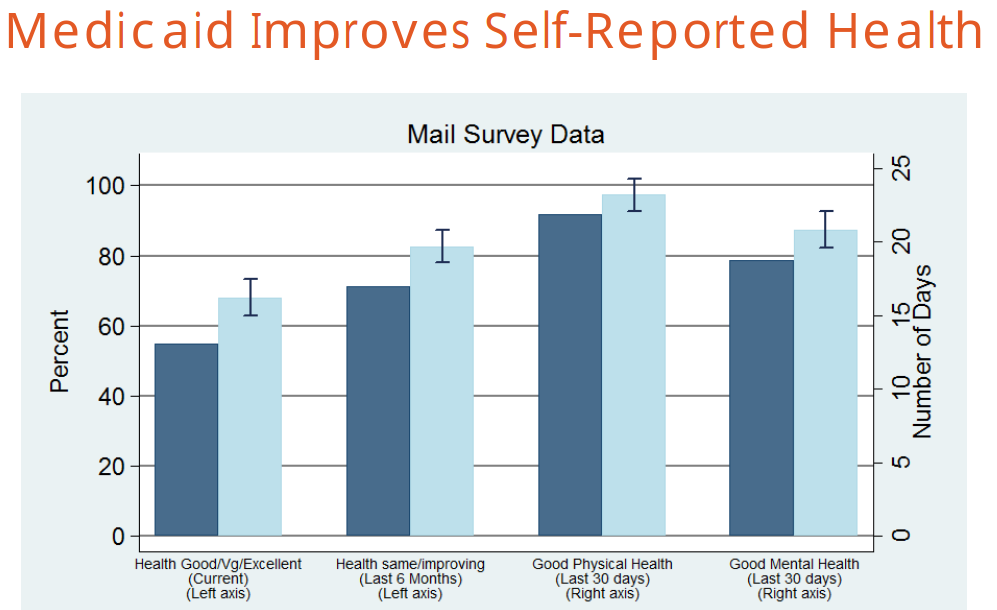
\includegraphics[width=\textwidth]{presentation-files/headlines/finkelstein-2019.png}
        \end{subfigure}
        \begin{subfigure}[c]{0.55\textwidth}
            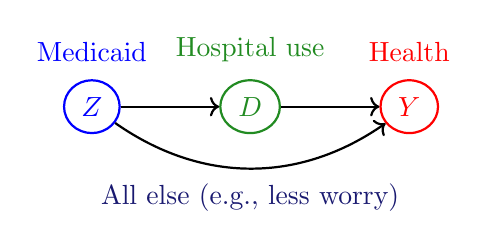
\begin{tikzpicture}
                \node[state, thick,ForestGreen] (mediator) at (0,0) {$D$};
                \node[state, thick,blue] (treatment) [left=1.25cm of mediator] {$Z$};
                \node[state, thick,red] (outcome) [right=1.25cm of mediator] {$Y$};
                % Label the nodes with econ examples
                \node[color=blue, above=0.1cm of treatment] {Medicaid};
                \node[color=red, above=0.1cm of outcome] {Health};
                \node[color=ForestGreen, above=0.1cm of mediator] {Hospital use};
                % Add in direct + indirect effects.
                %\path[->,thick] (treatment) edge[bend right=45] (outcome);
                % Label the pathways with the colours
                \path[->, thick] (treatment) edge (mediator);
                \path[->, thick] (mediator) edge (outcome);
                \path[->, thick] (treatment) edge[bend right=35] (outcome);
                \node[color=MidnightBlue, below=0.5cm of mediator] {All else (e.g., less worry)};
            \end{tikzpicture}
        \end{subfigure}
    \end{figure}
    Consider the case \textbf{individuals go to the hospital} to maximise health.
    \[ D_i \left( z' \right) = \indicator{
        \underbrace{Y_i\left( z', 1 \right) - Y_i\left( z', 0 \right)}_{\text{Benefits}}
        \geq \underbrace{C_i}_{\text{Costs}}}, \;\;\; \text{for } z'=0,1.
    \]
    i.e., Roy (1951) selection into $D_i$.
\end{frame}
%-------------------------------------------------------------------------------
\begin{frame}[noframenumbering]
    \frametitle{Direct \& Indirect Effects --- Selection} 
    \colorbox{yellow}{\textbf{SI:}
        Hospital usage is quasi-random, conditional on Medicaid assignment} \\
    \colorbox{yellow}{$Z_i$ and demographics $\vec X_i$.}

    \vskip0.25cm
    Consider the case \textbf{individuals go to the hospital} to maximise health.
    \[ D_i \left( z' \right) = \indicator{
        \underbrace{Y_i\left( z', 1 \right) - Y_i\left( z', 0 \right)}_{\text{Benefits}}
        \geq \underbrace{C_i}_{\text{Costs}}}, \;\;\; \text{for } z'=0,1.
    \]
    i.e., Roy (1951) selection into $D_i$.
    \par\noindent\rule{\textwidth}{0.4pt}
    \vfill
    \textbf{Theorem:}
    If selection is Roy-style, and benefits are not 100\% explained by $Z_i, \vec X_i$, then \textbf{SI} does not hold.

    \vskip0.125cm
    \textbf{Proof sketch:} suppose $D_i$ is ignorable $\implies$ selection-into-$D_i$ is explained 100\% by $\left\{ C_i, Z_i, \vec X_i \right\}$, while unobserved gains explain 0\%.
\end{frame}
%-------------------------------------------------------------------------------
\begin{frame}[noframenumbering]
    \frametitle{Direct \& Indirect Effects --- Selection} 
    \colorbox{yellow}{\textbf{SI:}
        Hospital usage is quasi-random, conditional on Medicaid assignment} \\
    \colorbox{yellow}{$Z_i$ and demographics $\vec X_i$.}

    \vskip0.25cm
    Consider the case \textbf{individuals go to the hospital} to maximise health.
    \[ D_i \left( z' \right) = \indicator{
        \underbrace{Y_i\left( z', 1 \right) - Y_i\left( z', 0 \right)}_{\text{Benefits}}
        \geq \underbrace{C_i}_{\text{Costs}}}, \;\;\; \text{for } z'=0,1.
    \]
    i.e., Roy (1951) selection into $D_i$.
    \par\noindent\rule{\textwidth}{0.4pt}
    $\implies$ unobserved confounder $\vec U$ \\
    e.g., underlying health conditions.
    \vskip-1.375cm
    \begin{figure}[h!]
        \centering
        \singlespacing
        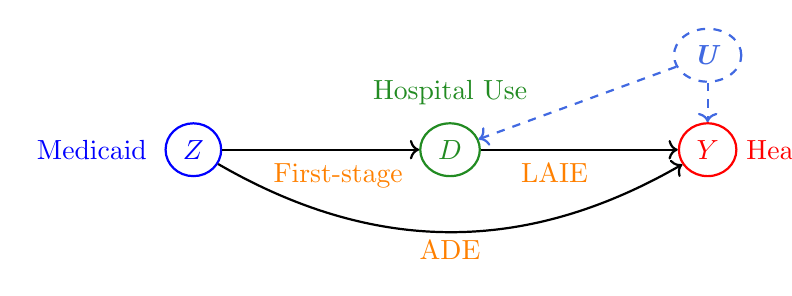
\begin{tikzpicture}
            \node[state, thick,ForestGreen] (mediator) at (0,0) {$D$};
            \node[state, thick,blue] (treatment) [left=2.5cm of mediator] {$Z$};
            \node[state, thick,red] (outcome) [right=2.5cm of mediator] {$Y$};
            % Label Z, D, Y
            \node[color=ForestGreen] [above=0.1cm of mediator] {Hospital Use};
            \node[color=blue] [left=0.1cm of treatment] {Medicaid};
            \node[text width=0.1cm, color=red] [right=-0.01cm of outcome] {Health};
            % Draw the causal arrows
            \path[->, thick] (treatment) edge (mediator);
            \path[->, thick] (mediator) edge (outcome);
            \path[->, thick] (treatment) edge[bend right=30] (outcome);
            % Label direct and indirect effect
            \node[color=orange] [below left=-0.2cm and 0.2cm of mediator] {First-stage};
            \node[color=orange] [below right=-0.2cm and 0.5cm of mediator] {LAIE};
            \node[color=orange] [below=0.675cm of mediator] {ADE};
            % Add in the confounders
            %\node[state, thick,RoyalPurple] (confounderX) [above=1.5cm of mediator] {$\vec{X}$};
            %\path[->,RoyalPurple] (confounderX) edge (mediator);
            %\node[color=RoyalPurple] [left=0.1cm of confounderX] {Observed controls};
            \node[state, thick,dashed,thick,RoyalBlue] (confounderU) [
                above=0.5cm of outcome] {$\vec U$};
            \path[->,thick,dashed,color=RoyalBlue] (confounderU) edge (mediator);
            \path[->,thick,dashed,color=RoyalBlue] (confounderU) edge (outcome);
            %\node[color=RoyalBlue] [right=0.1cm of confounderU] {Unobserved confounder};
        \end{tikzpicture}
    \end{figure}
\end{frame}
%-------------------------------------------------------------------------------
\begin{frame}[noframenumbering]
    \frametitle{Direct \& Indirect Effects --- Selection}
    In practice, the only way to believe the \textbf{SI} assumption (selection-on-observables) is to study a case with another natural experiment for $D_i$ --- in addition to the one that guaranteed $Z_i$ is ignorable.
    \vskip-0.5cm
    \begin{figure}[h!]
        \centering
        \singlespacing
        \begin{subfigure}[c]{0.475\textwidth}
            \centering
            \caption{Cells in a lab
                $\to$ \textbf{SI} believable.}
            
\includegraphics[width=\textwidth]{
                presentation-files/headlines/science-lab.png}
        \end{subfigure}
        \begin{subfigure}[c]{0.475\textwidth}
            \centering
            \caption{People choosing healthcare
                $\to$ \textbf{SI} not.}
            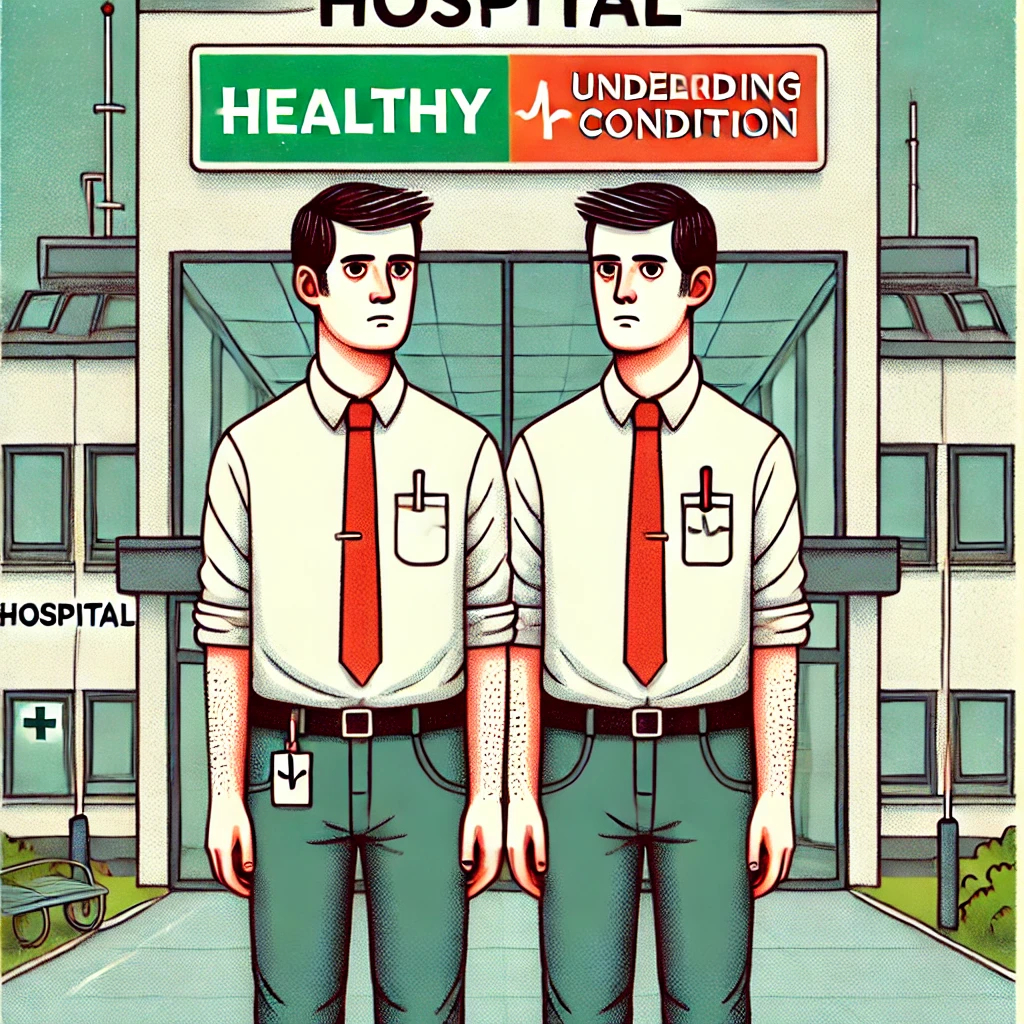
\includegraphics[width=\textwidth]{
                presentation-files/headlines/health-differences.jpg}
        \end{subfigure}
    \end{figure}
\end{frame}
%-------------------------------------------------------------------------------
\begin{frame}
    \frametitle{Direct \& Indirect Effects --- Selection Bias}
    \begin{itemize}
        \item What happens if you go ahead and estimate CM anyway?
        \item Would this be problematic?
        \item Estimating causal effects with an unobserved confounder is usually quite bad$\hdots$.
    \end{itemize}
    \par\noindent\rule{\textwidth}{0.4pt}
    \vskip0.25cm
    \textbf{Definition:} Selection bias (Heckman Ichimura Smith Todd, 1998).
    \vskip0.25cm
    Estimating $Z \to Y$, if $Z$ not ignorable:
    \begin{align*}
        &\Egiven{ Y_i}{Z_i =1} - \Egiven{ Y_i}{Z_i =0} \\
        &= \text{ATT} \\
        &\;\;\;\; + \underbrace{\Big(
            \Egiven{ Y_i(0,.)}{Z_i =1} - \Egiven{ Y_i(0,.)}{Z_i =0} \Big)}_{
                \text{Selection Bias}}.
    \end{align*}
    \vskip1.125cm
\end{frame}
%-------------------------------------------------------------------------------
\begin{frame}[noframenumbering]
    \frametitle{Direct \& Indirect Effects --- Selection Bias}
    \begin{itemize}
        \item What happens if you go ahead and estimate CM anyway?
        \item Would this be problematic?
        \item Estimating causal effects with an unobserved confounder is usually quite bad$\hdots$.
    \end{itemize}
    \par\noindent\rule{\textwidth}{0.4pt}
    \vskip0.25cm
    \textbf{Definition:} Selection bias (Heckman Ichimura Smith Todd, 1998).
    \vskip0.25cm
    Estimating $Z \to Y$, if $Z$ not ignorable:
    \begin{align*}
        &\Egiven{ Y_i}{Z_i =1} - \Egiven{ Y_i}{Z_i =0} \\
        &= \text{ATE} \\
        &\;\;\;\; + \underbrace{\Big(
            \Egiven{ Y_i(0,.)}{Z_i =1} - \Egiven{ Y_i(0,.)}{Z_i =0} \Big)}_{
                \text{Selection Bias}} \\
        &\;\;\;\;+ \underbrace{ \Prob{Z_i=0} (\text{ATT}- \text{ATU}) }_{
            \text{Group-differences Bias}}.
    \end{align*}
\end{frame}
%-------------------------------------------------------------------------------
\begin{frame}
    \frametitle{Direct \& Indirect Effects --- Selection Bias}
    $\implies$ CM Effects have this same flavour, causal effects contaminated by (less interpretable) bias terms.
    \[ \text{\textcolor{purple}{CM Estimand}}
        = \text{\textcolor{blue}{ADE}}
            + \Big(\text{\textcolor{red}{Selection Bias}}
            + \text{\textcolor{orange}{Group difference bias}}\Big) \]
    \vspace{-0.25cm}
    {\footnotesize
    \begin{align*}
        & \underbrace{\mathbb E_{D_i} \Big[
            \Egiven{Y_i}{Z_i = 1, D_i} - \Egiven{Y_i}{Z_i = 0, D_i} \Big]}_{
                \text{\textcolor{purple}{Estimand, Direct Effect}} } \\
        & = \underbrace{\E{Y_i(1, D_i(Z_i)) - Y_i(0, D_i(Z_i))}}_{
            \text{\textcolor{blue}{Average Direct Effect}}} \\
        & \;\;\;\; + \underbrace{ \mathbb E_{D_i} \Big[ 
            \Egiven{Y_i(0, D_i(Z_i))}{D_i(1) = d} 
            - \Egiven{Y_i(0, D_i(Z_i))}{D_i(0) = d} \Big] }_{
                \text{\textcolor{red}{Selection Bias}}} \\
        & \;\;\;\; + \underbrace{ \E[D_i ]{
            \begin{aligned}
            &\Big(1 - \Prob{D_i(1) = d} \Big) \\
            &\times \left( \begin{aligned}
                &\Egiven{Y_i(1, D_i(Z_i)) - Y_i(0, D_i(Z_i))}{D_i(1) = 1-d} \\ 
                &  - \Egiven{Y_i(1, D_i(Z_i)) - Y_i(0, D_i(Z_i))}{D_i(0) = d}
                \end{aligned} \right) \end{aligned}} }_{
                    \text{\textcolor{orange}{Group difference bias}}}
    \end{align*}}
\end{frame}
%-------------------------------------------------------------------------------
\begin{frame}
    \frametitle{Direct \& Indirect Effects --- Selection Bias}
    $\implies$ CM Effects have this same flavour, causal effects contaminated by (less interpretable) bias terms.
    Put $\pi = \Prob{D_i(1) = 1, D_i(0) = 0}$.
    \[ \text{\textcolor{purple}{CM Estimand}}
        = \text{\textcolor{ForestGreen}{AIE}}
            + \Big(\text{\textcolor{red}{Selection Bias}}
            + \text{\textcolor{orange}{Group difference bias}}\Big) \]
    \vspace{-0.25cm}
    {\footnotesize
    \begin{align*}
        & \underbrace{\E[Z_i]{
            \Big( \Egiven{D_i}{Z_i = 1} - \Egiven{D_i}{Z_i = 0} \Big) \times
            \Big( \Egiven{Y_i}{Z_i, D_i = 1} - \Egiven{Y_i}{Z_i, D_i = 0} \Big) }}_{ \text{\textcolor{purple}{Estimand, Indirect Effect}} } \\
        & = \underbrace{\E{Y_i(Z_i, D_i(1)) - Y_i(Z_i, D_i(0))}}_{
            \text{\textcolor{ForestGreen}{Average Indirect Effect}} } \\
        & \;\;\;\; + \underbrace{\pi  \Big(
            \Egiven{Y_i(Z_i, 0)}{D_i = 1} - \Egiven{Y_i(Z_i, 0)}{D_i = 0} \Big)}_{
                \text{\textcolor{red}{Selection Bias}}} \\
        %& \;\;\;\; + \Prob{D_i(1) = 1, D_i(0) = 0} \times \\
        %& \;\;\;\; \;\; \underbrace{ \left[ \begin{aligned}
        & \;\;\;\; + \underbrace{ \pi \left[ \begin{aligned}
            &\Big( 1 - \Prob{D_i=1} \Big)
            \left( \begin{aligned}
                &\Egiven{Y_i(Z_i, 1) - Y_i(Z_i, 0)}{D_i = 1} \\ 
                &  - \Egiven{Y_i(Z_i, 1) - Y_i(Z_i, 0)}{D_i = 0}
            \end{aligned} \right) \\
            &+ \left( \frac{1 - \Prob{D_i(1) = 1, D_i(0) = 0} }{
                \Prob{D_i(1) = 1, D_i(0) = 0}} \right)
            \left( \begin{aligned}
                &\Egiven{Y_i(Z_i, 1) - Y_i(Z_i, 0)}{D_i(1) = 0 \text{ or } D_i(0)=1} \\ 
                &  - \E{Y_i(Z_i, 1) - Y_i(Z_i, 0)}
            \end{aligned} \right)
        \end{aligned} \right]}_{\text{\textcolor{orange}{Groups difference Bias}}}
    \end{align*}}
\end{frame}
%-------------------------------------------------------------------------------
\section{2. Identification by Selection Model}
%-------------------------------------------------------------------------------
\begin{frame}
    \frametitle{Identification}
    How do economists think about estimating treatment effects in these systems?
    \begin{enumerate}
        \item Estimate the ATE, and call it a day.
        \item (optional) Present suggestive evidence of mechanisms$\hdots$.
    \end{enumerate}

    See Blackwell Matthew Ruofan Opacic (2024).

    Put a button here, linking to the current economic approach and screenshot the abstract of Carvahlo (2024).
\end{frame}
%-------------------------------------------------------------------------------
\end{document}
